\documentclass[10pt,a4paper]{article}
\usepackage[left=18mm,right=18mm,top=17mm,bottom=17mm]{geometry}
\usepackage{fontspec,xeCJK}
\usepackage{graphicx,array,tabularx,booktabs,fvextra}
\setmainfont{Times New Roman}
\setCJKmainfont{SimSun}[BoldFont=SimHei]
\setmonofont{Consolas}
\setCJKmonofont{SimSun}
\setlength\parindent{0pt}
\setlength\parskip{5pt}
\pagestyle{plain}
\renewcommand{\arraystretch}{1.24}
\newcolumntype{L}{>{\raggedright\arraybackslash}X}
\newcommand{\heading}[2]{%
  {\small #1}\par\vspace{2pt}%
  {\LARGE\bfseries #2}\par\vspace{7pt}}
\newcommand{\sqltitle}[2]{\par\noindent{\small\bfseries #1\quad #2}\par}
\begin{document}
\heading{CS307 / 2026 年秋季 / 项目一}{深圳地铁数据库}
{\large\bfseries 组员信息与分工}\par
实验班：周一下午78节

\begin{tabularx}{\linewidth}{@{}p{39mm}LL@{}}
\toprule
\textbf{任务} & \textbf{Zhong Haozhe（A）} & \textbf{Guo Liangyue（B）}\\
\midrule
学号 & 12510615 & 12513012\\
Task 1 · 概念 ER 图 & 绘制 ER 图并注明绘图工具 & —\\
Task 2 · 数据库设计 & — & 编写 DDL，导出数据库关系图，说明表和字段，检查范式与约束\\
Task 3.1 · 脚本与 AI & 汇总脚本、运行方法和 AI 使用情况 & 提供自己的使用记录和临时导入方法\\
Task 3.2 · 一键导入 & 转换数据、生成导入 SQL、验证重跑及数据完整性 & —\\
Task 3.3 · 数据核验 & Q1、Q3、Q5、Q6（车站总数、各区运营站数、出口最多车站、地标前缀） & Q2、Q4、Q7（线路总数、按开通年份统计、前后第 \(n\) 站函数）\\
Task 4 · 车站管理 & 添加、修改、删除、查询车站 & —\\
Task 4 · 线路管理 & — & 添加、修改、删除、查询线路\\
Task 4 · 站线关系 & — & 在指定位置插入一个或多个站，从线路移除车站\\
Task 4 · 两站路径 & — & 查询两站路径，提供调用接口\\
Task 4 · 两地标路线 & 匹配地标、关联车站、调用路径接口并整理结果 & 提供路径查询接口\\
Task 4 · 票价查询 & 实现票价查询 & —\\
Task 4 · 用户界面 & 设计界面并接入双方功能 & 提供所负责功能的调用接口\\
Task 4 · 架构与启动 & 按统一接口接入所负责的模块 & 设计整体架构、公共数据库连接及统一入口\\

\bottomrule
\end{tabularx}

两人共同确定数据库模型、站序规则和功能接口，各自负责所分配模块的测试和报告内容，并使用正式导入脚本重建数据库后联调。

\clearpage
\heading{Task 1}{概念 ER 图}
使用 draw.io Desktop 32.6.10 绘制。出口是弱实体，由所属车站和部分键 \texttt{exit\_code} 共同识别。
\begin{center}
\includegraphics[height=.78\textheight,width=\linewidth,keepaspectratio]{../DB_project_Repo/Task1/source/Metro_ER_Diagram.drawio.png}

图 1\quad 深圳地铁数据库的概念 ER 图
\end{center}

\clearpage
\heading{Task 2}{数据库设计}
根据两份 CSV 在 PostgreSQL 的 \texttt{public} 模式中建立七张表。567 条站线记录对应 439 个车站、29 条线路和 10 个行政区。

\begin{minipage}[t]{.47\linewidth}
\vspace{0pt}
\centering
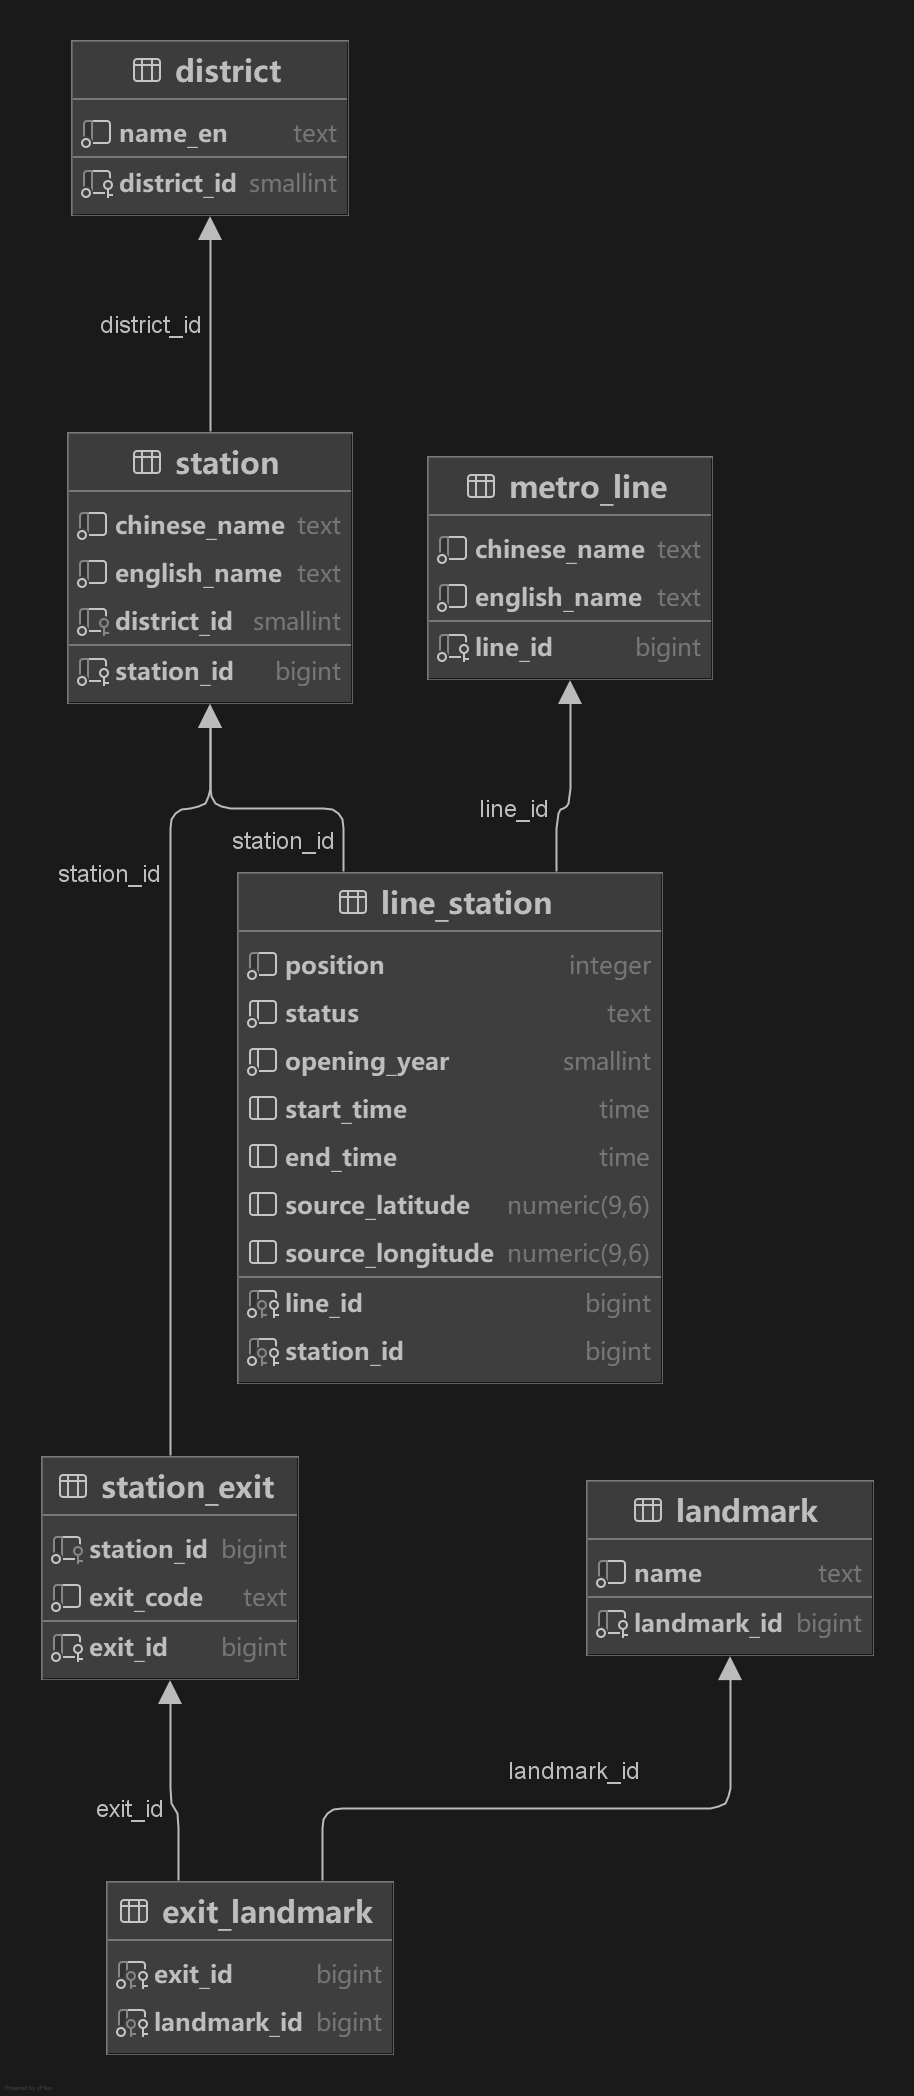
\includegraphics[width=\linewidth,height=.76\textheight,keepaspectratio]{DataGrip-gray.png}

\small 图 2\quad DataGrip 导出的数据库关系图
\end{minipage}\hfill
\begin{minipage}[t]{.48\linewidth}
\vspace{0pt}
\textbf{实体与关系}\par
一个行政区可包含多个车站。车站与线路通过 \texttt{line\_station} 建立多对多关系。一个车站可有多个出口，出口与地标名称通过 \texttt{exit\_landmark} 建立多对多关系。图中箭头由持有外键的子表指向被引用的父表。七张表均参与外键关系，且外键方向无环。

\textbf{业务键与属性归属}\par
车站以中文名和行政区作为业务唯一键，不同区的梨园站分别保留，英文站名允许重名。线路的中英文名称分别唯一。站序、运营状态、开通年份、首末班时间和原始坐标存于站线关系表，以保留同一车站在不同线路上的属性差异。

\textbf{三范式}\par
第一范式。字段保存单值，地标列表按中文逗号拆成独立名称，再用关联表建立联系。\par
第二范式。站线属性依赖完整的站线组合键，出口地标关联表仅含复合主键字段。\par
第三范式。行政区、线路和地标名称各自保存在实体表中。关系表通过外键引用这些实体，避免非键属性之间的传递依赖。

\textbf{扩展与约束}\par
内部编号保持稳定，改名时无需改动关联关系。新增线路、车站或地标关联可通过增加记录完成。图中钥匙图标标记主键，具体字段与约束见下一页。
\end{minipage}

\clearpage
\heading{Task 2}{表、字段与完整性约束}
表中 PK 表示主键，FK 表示外键，UQ 表示唯一约束。实体编号使用 \texttt{GENERATED BY DEFAULT AS IDENTITY}，行政区编号为 \texttt{SMALLINT}，其余为 \texttt{BIGINT}。文本字段使用 \texttt{TEXT}。

\begin{tabularx}{\linewidth}{@{}p{33mm}L@{}}
\toprule
\textbf{表名与用途} & \textbf{字段与约束}\\
\midrule
\texttt{district}\newline 行政区 &
\texttt{district\_id} 为 PK；\texttt{name\_en} 保存英文区名，设 UQ。\\
\addlinespace
\texttt{station}\newline 车站 &
\texttt{station\_id} 为 PK；\texttt{chinese\_name}、\texttt{english\_name} 保存中英文站名；\texttt{district\_id} 为指向行政区的 FK。中文站名与行政区的组合设 UQ。\\
\addlinespace
\texttt{metro\_line}\newline 线路及单独命名的延长线 &
\texttt{line\_id} 为 PK；\texttt{chinese\_name}、\texttt{english\_name} 保存中英文线路名，各自设 UQ。\\
\addlinespace
\texttt{line\_station}\newline 站线关系 &
\texttt{line\_id}、\texttt{station\_id} 分别指向线路和车站，共同构成 PK。\texttt{position} 为正整数站序，与 \texttt{line\_id} 组成可延迟检查的 UQ。\texttt{status} 为运营或建设状态，\texttt{opening\_year} 为实际或预计开通年份。\texttt{start\_time}、\texttt{end\_time} 保存首末班时间，类型为 \texttt{TIME WITHOUT TIME ZONE}。\texttt{source\_latitude}、\texttt{source\_longitude} 保留原始坐标，类型为 \texttt{NUMERIC(9,6)}。\\
\addlinespace
\texttt{station\_exit}\newline 车站出口 &
\texttt{exit\_id} 为 PK；\texttt{station\_id} 为指向车站的 FK；\texttt{exit\_code} 保存出口编号。车站与出口编号的组合设 UQ。\\
\addlinespace
\texttt{landmark}\newline 地标名称 &
\texttt{landmark\_id} 为 PK；\texttt{name} 保存拆分并去除首尾空白后的地标名称，设 UQ。\\
\addlinespace
\texttt{exit\_landmark}\newline 出口地标关系 &
\texttt{exit\_id}、\texttt{landmark\_id} 分别指向出口和地标，共同构成 PK。\\
\bottomrule
\end{tabularx}

\textbf{完整性与源数据处理}\par
除首末班时间与原始坐标外，其余字段均为必填。必填文本通过检查约束拒绝空白。全部外键采用 \texttt{ON DELETE RESTRICT} 与 \texttt{ON UPDATE RESTRICT}。开通年份须为正值，站序连续性由应用事务维护。索引覆盖站名、行政区、关系反向查询及地标前缀查询。

空时间与空坐标映射为 \texttt{NULL}。

独立附件 \texttt{Task2/create\_table.sql} 含全部七张表的建表语句、约束和索引，与生成一键导入脚本使用的 DDL 一致。

\clearpage
\heading{Task 3.1}{数据导入脚本与 AI 使用}
\begin{tabularx}{\linewidth}{@{}>{\raggedright\arraybackslash}p{46mm}p{18mm}p{28mm}L@{}}
\toprule
\textbf{名称} & \textbf{类型} & \textbf{作者或使用者} & \textbf{用途及运行方法}\\
\midrule
\texttt{ImportSqlGenerator.}\allowbreak\texttt{java} & Java 脚本 & Zhong Haozhe & 读取两份 CSV，整理数据并生成 \texttt{import.sql}。在 IntelliJ IDEA 中运行，以仓库根目录为程序参数。\\
\addlinespace
\texttt{create\_table.sql} & SQL 脚本 & Guo Liangyue & 定义表、约束和索引。生成器读取该文件，将语句写入一键导入脚本。\\
\addlinespace
\texttt{import.sql} & 生成的 SQL & 由 Zhong Haozhe 的 Java 程序生成 & 删除旧项目表、重建表并批量插入数据。在 DataGrip 连接目标 PostgreSQL 数据库，执行整个文件。\\
\addlinespace
OpenAI Codex（GPT-6.1 Terra） & AI 编码工具 & Zhong Haozhe & 辅助规划生成器的结构，编写、修改和解释生成器代码。\\
\bottomrule
\end{tabularx}

\clearpage
\heading{Task 3.3 / Data Accuracy Checking}{数据准确性检查}

\sqltitle{Q1}{车站总数}
\begin{Verbatim}[fontsize=\small,breaklines=true,breakanywhere=true,breaksymbolleft={}]
select count(*) as station_count from public.station;
\end{Verbatim}
\sqltitle{Q2}{线路总数}
\begin{Verbatim}[fontsize=\small,breaklines=true,breakanywhere=true,breaksymbolleft={}]
select count(distinct line_id) from public.metro_line;
\end{Verbatim}
\sqltitle{Q3}{按行政区统计运营站点}
\begin{Verbatim}[fontsize=\small,breaklines=true,breakanywhere=true,breaksymbolleft={}]
select d.name_en as district, count(s.station_id) as station_count
from public.district d
left join public.station s on s.district_id = d.district_id
    and exists (select 1 from public.line_station ls
                where ls.station_id = s.station_id and ls.status = 'Operation')
group by d.district_id, d.name_en
order by d.name_en;
\end{Verbatim}
\sqltitle{Q4}{指定线路各年开通站点数}
\begin{Verbatim}[fontsize=\small,breaklines=true,breakanywhere=true,breaksymbolleft={}]
select opening_year, count(*) cnt
from line_station
where line_id = (select line_id from metro_line where english_name=${line_name})
group by opening_year
order by opening_year;
\end{Verbatim}
\sqltitle{Q5}{指定线路出口最多的车站}
\begin{Verbatim}[fontsize=\small,breaklines=true,breakanywhere=true,breaksymbolleft={}]
with exit_counts as (
    select s.station_id, s.english_name, count(e.exit_id) as exit_count
    from public.metro_line l
    join public.line_station ls on ls.line_id = l.line_id
    join public.station s on s.station_id = ls.station_id
    left join public.station_exit e on e.station_id = s.station_id
    where l.english_name = 'Line 1'
    group by s.station_id, s.english_name
)
select english_name, exit_count from exit_counts
where exit_count = (select max(exit_count) from exit_counts)
order by english_name, station_id;
\end{Verbatim}
\sqltitle{Q6}{按地标前缀查询站点与出口}
\begin{Verbatim}[fontsize=\small,breaklines=true,breakanywhere=true,breaksymbolleft={}]
select s.chinese_name, d.name_en as district, e.exit_code, m.name as landmark
from public.landmark m
join public.exit_landmark em on em.landmark_id = m.landmark_id
join public.station_exit e on e.exit_id = em.exit_id
join public.station s on s.station_id = e.station_id
join public.district d on d.district_id = s.district_id
where m.name like '塘朗%'
order by s.english_name, d.name_en, s.chinese_name, e.exit_code, m.name;
\end{Verbatim}
\clearpage
\heading{Task 3.3 / Data Accuracy Checking}{前后第 \textit{n} 站}
\sqltitle{Q7}{查询指定车站前后第 \textit{n} 站}
\begin{Verbatim}[fontsize=\small,breaklines=true,breakanywhere=true,breaksymbolleft={}]
CREATE OR REPLACE function public.get_station_n_neighbor(
    station_name text, line_name text, n integer)
    returns setof text
    language plpgsql
as
$$
declare
    prename  text;
    nextname text;
begin
    if n isnull or n < 0 then
        raise exception 'n无效' using errcode = '22023';
    end if;
    with t1 as (select station_id, position, english_name
                from (select station_id, position
                      from public.line_station
                      where line_id = (select line_id
                                       from public.metro_line
                                       where english_name = line_name)) as t
                         natural left join public.station),
         t2 as (select position, english_name
                from t1
                where english_name = station_name)
    select pre_name, after_name
    into strict prename,nextname
    from (
             t2
             left join (select position, english_name as pre_name from t1) as t3
               on t2.position = t3.position::bigint + n
             left join (select position, english_name as after_name from t1) as t4
               on t2.position = t4.position::bigint - n
             );
    return next prename;
    return next nextname;
    return;
EXCEPTION
    WHEN NO_DATA_FOUND THEN
        RAISE EXCEPTION
            '线路 % 不存在，或站点 % 不在这条线路上',
            line_name, station_name using errcode = 'P0002';
    WHEN TOO_MANY_ROWS THEN
        RAISE EXCEPTION
            '线路 % 内有多个英文名为 % 的车站，无法唯一定位',
            line_name, station_name using errcode = 'P0003';
end;
$$;
select * from get_station_n_neighbor('Mawan','Line 5',3);
\end{Verbatim}
\end{document}

